\subsection{Evolution of the program (Roar)}

The program was developed in four main steps. These steps are outlined in figure \ref{fig:PE}.

\begin{figure}[H]
    \centering
    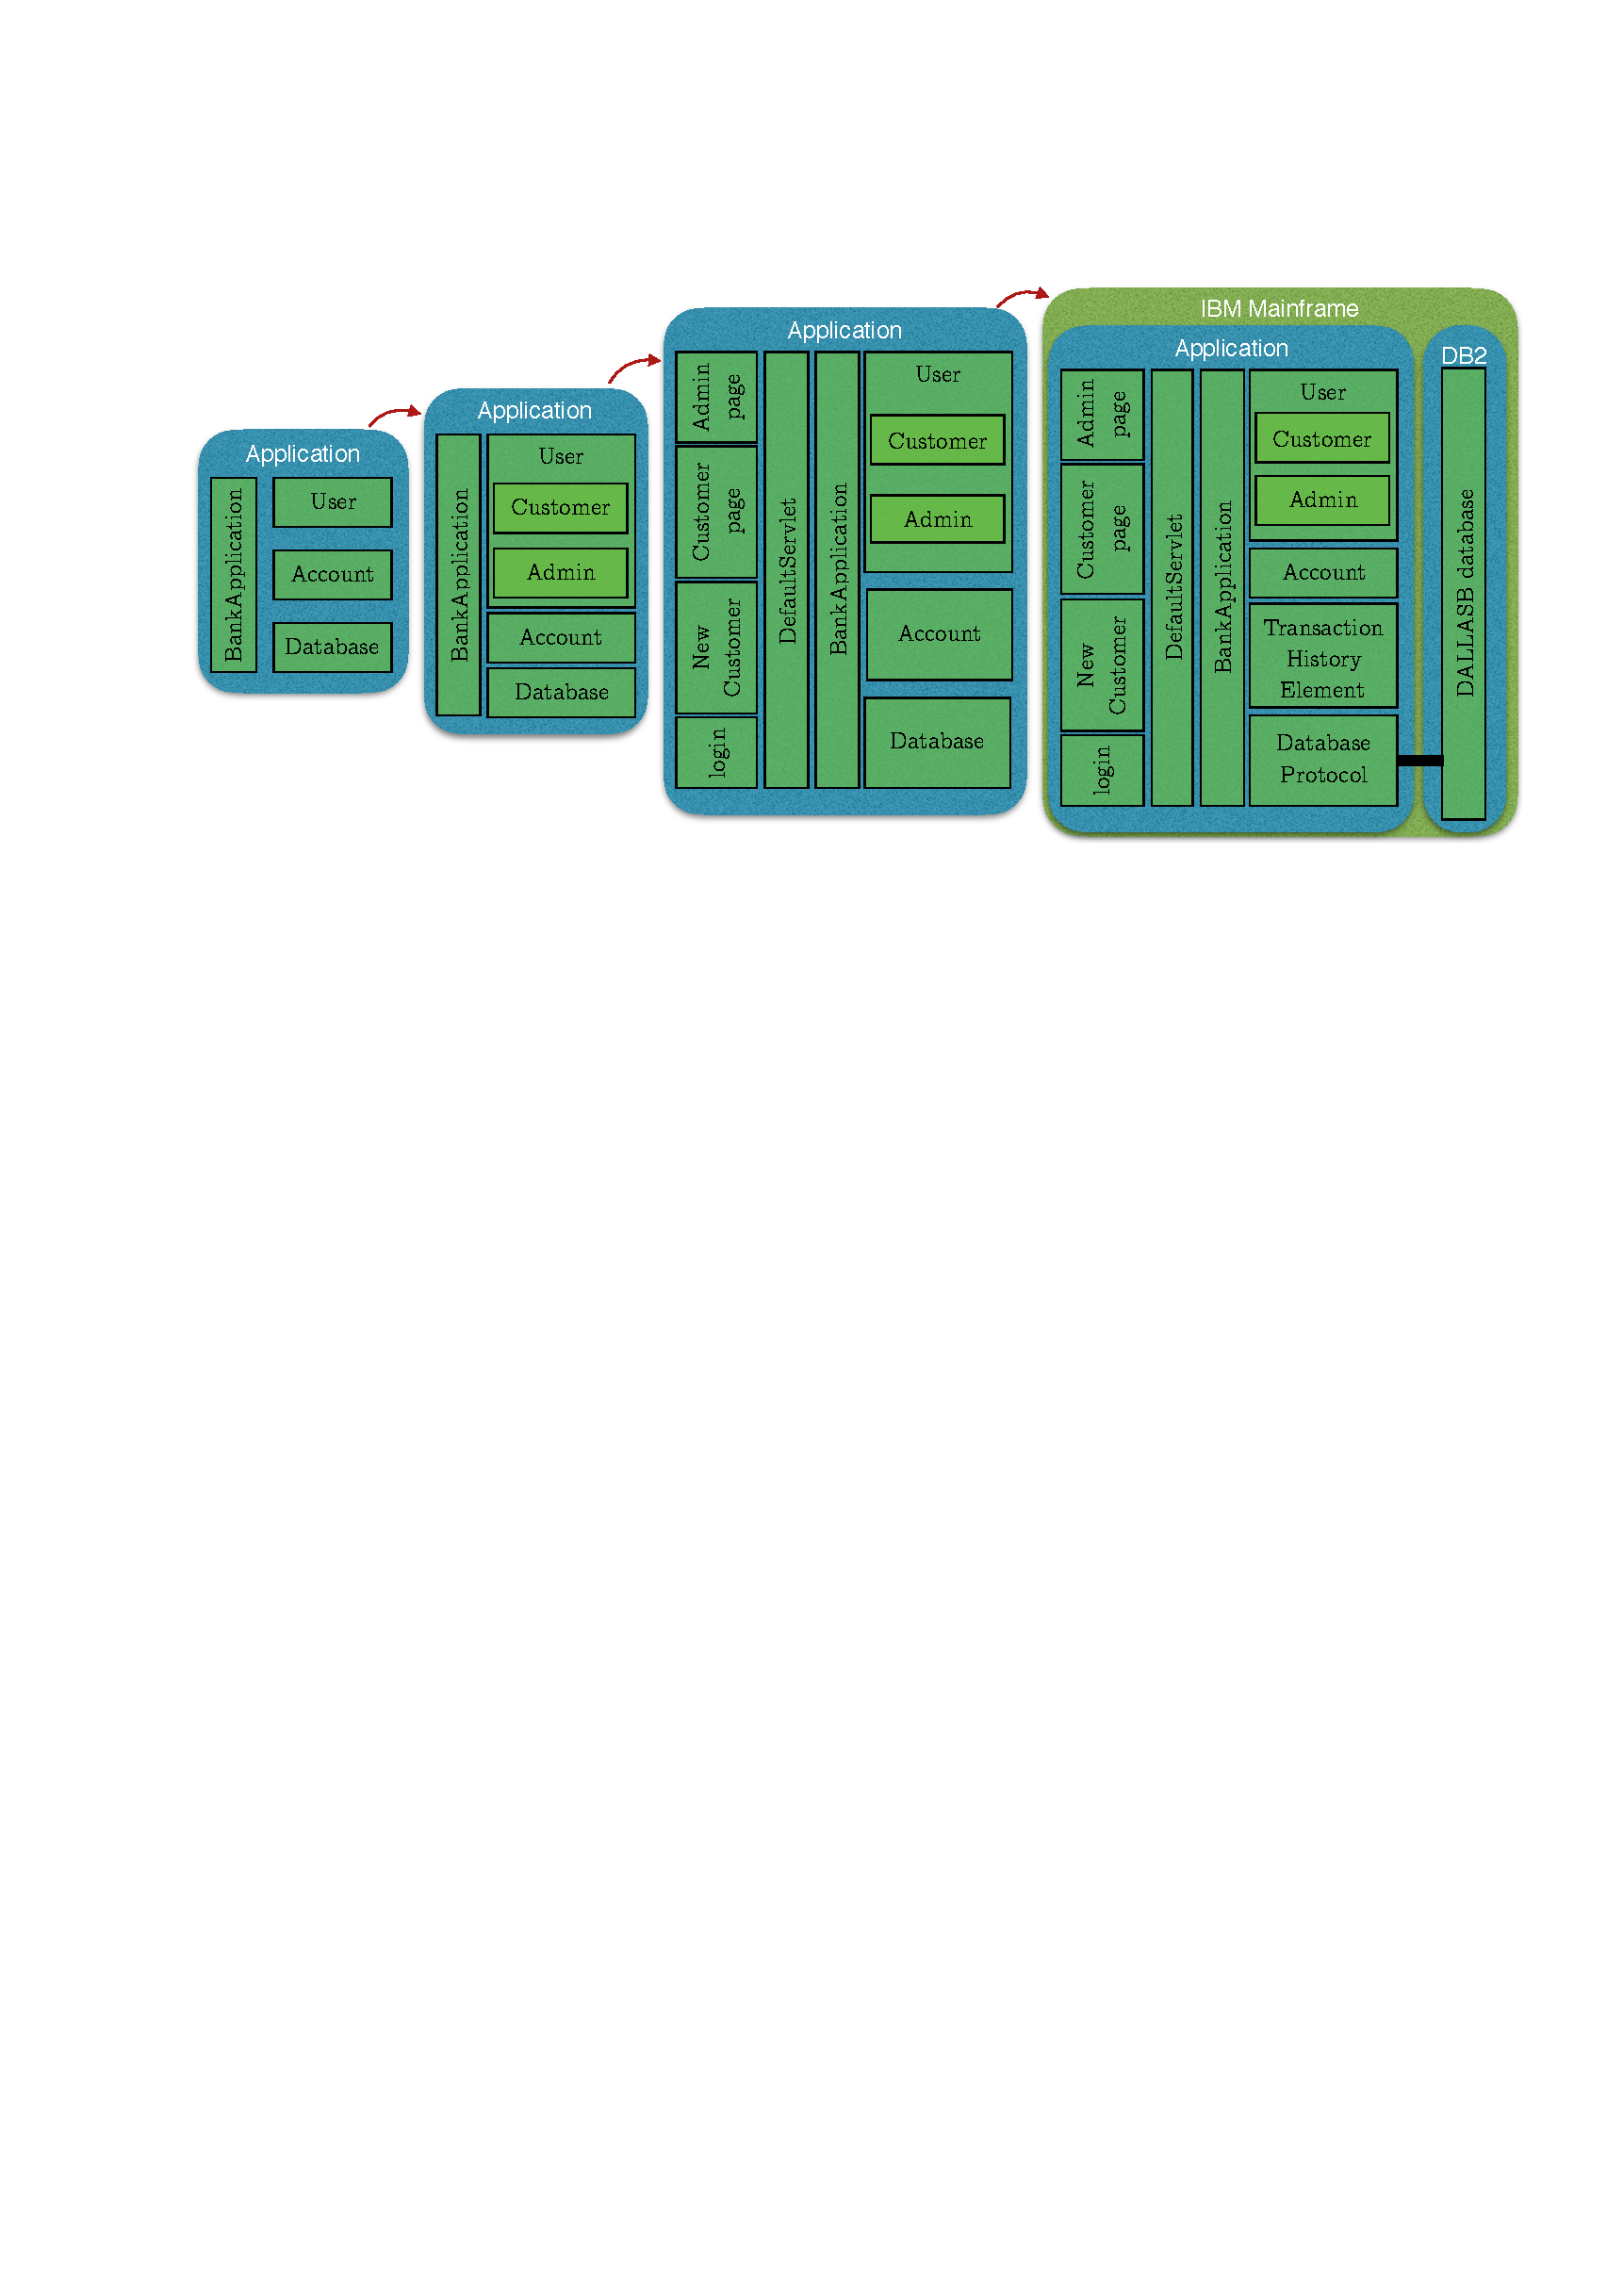
\includegraphics[width=\textwidth]{figures/PE}
    \caption{Outline of the four main stages of the program. At every stage the we had a fully working program, our development structure was inspired by agile development.}
    \label{fig:PE}
\end{figure}

\textbf{Stage 1:} At first, the program was comprised of the classes: \texttt{BankApplication}, \texttt{User}, \texttt{Account} and an auxiliary class called \texttt{Database}. These were implemented as the core of the program, with the \texttt{User} and \texttt{Account} as the model and \texttt{BankApplication} as the controller. The \texttt{Database} class's only purpose was to simulate the interaction with the database. No UI was created at this point, since the application was tested with direct method calls. Since the tools needed to connect the program with e.g. the database was not granted from the start of the course, this made it possible to encapsulate what the heart of the program was and test our ideas.

\textbf{Stage 2:} The next big step was to divide (or rather extend) the users into customers and admins. This made it possible to distinguish between customers and admins when features were allowed to one but not the other.

\textbf{Stage 3:} Then the application was made to run on a Java servlet, turning the application into a web application. The servlet was implemented in the \texttt{DefaultServer} class, and was the main link between the user and the application. \texttt{BankApplication}, whose main job is to alter the model, was not changed. Instead the \texttt{DefaultServer}'s job was made to convert the user input into the apropriate tasks for the \texttt{BankApplication} to carry out. With the DefaultServlet implemented, the next step was to create the UI from which the user interacts through. At first the UI was implemented through simple HTML files, but as more logic was needed in the separate pages, they all got converted into JSP files. This made them able to run Java code, as well as HTML and CSS code. 

\textbf{Stage 4:} When the database connection was implemented, the \texttt{Database} class was substituted with a class called \texttt{DatabaseProtocol}. This class contained the same features as the \texttt{Database} class, but instead of local storage in arrays, the data was stored in the DALLASB database delivered by IBM. Once the database was connected, the design of the program, was as planned, and has changed very little during the subsequent sessions. 

Besides the mentioned classes, some auxiliary classes were created. The exception classes help control the dataflow, when unwanted behavior is encountered. Also a wrapper class called \texttt{TransactionHistoryElement} for data transfer was written.